\documentclass[pdf]{beamer}

\usepackage{listings}
\usepackage{tikz}

\usetheme{Boadilla}

\usetikzlibrary{shapes, arrows}

\tikzstyle{blank} = [node distance=1.0cm]
\tikzstyle{block} = [rectangle, text centered, rounded corners,
                     minimum height=0.5cm, node distance=1.0cm,
                     thick, draw=blue!50,
                     fill=blue!20]
\tikzstyle{block-emph} = [block, draw=red!50, fill=red!20]
\tikzstyle{block-neutral} = [block, draw=black!50, fill=black!20]
\tikzstyle{line} = [draw, -latex']

\definecolor{keywords}{RGB}{220,0,90}
\definecolor{strings}{RGB}{0,140,0}
\definecolor{comments}{RGB}{0,127,0}
\definecolor{identifiers}{RGB}{20,20,75}

\lstset{
    basicstyle=\ttfamily\small, 
    basewidth = .48em,
    escapeinside=@@}

\title{An Observable OCaml}
\subtitle{Compiling OCaml into C}
\author{Tianlin Zhang}
\date{5th February, 2018}

\begin{document}

\begin{frame}
\titlepage
\end{frame}

\iffalse

\begin{frame}[fragile]{Introduction}
\begin{lstlisting}[language=Caml,
keywordstyle=\color{keywords},
commentstyle=\color{comments},
stringstyle=\color{strings},
showstringspaces=false,
identifierstyle=\color{identifiers}]
(* val intersperse : 'a -> 'a list -> 'a list *)
let intersperse x ys =
  let rec go = function
    | [y] -> [y]
    | [] -> []
    | y :: ys -> y :: x :: go ys
  in go ys

(* val add_newlines : string list -> string list *)
let add_newlines = intersperse "\n"
\end{lstlisting}
\pause
Challenges of compiling OCaml to C:
\begin{itemize}
    \pause
    \item polymorphism
    \pause
    \item first class functions
    \pause
    \item lexical closures
    \pause
    \item partial application
    \pause
    \item algebraic data types
\end{itemize}
\end{frame}

\fi

\begin{frame}{Structure of the project}
\begin{figure}
{\small
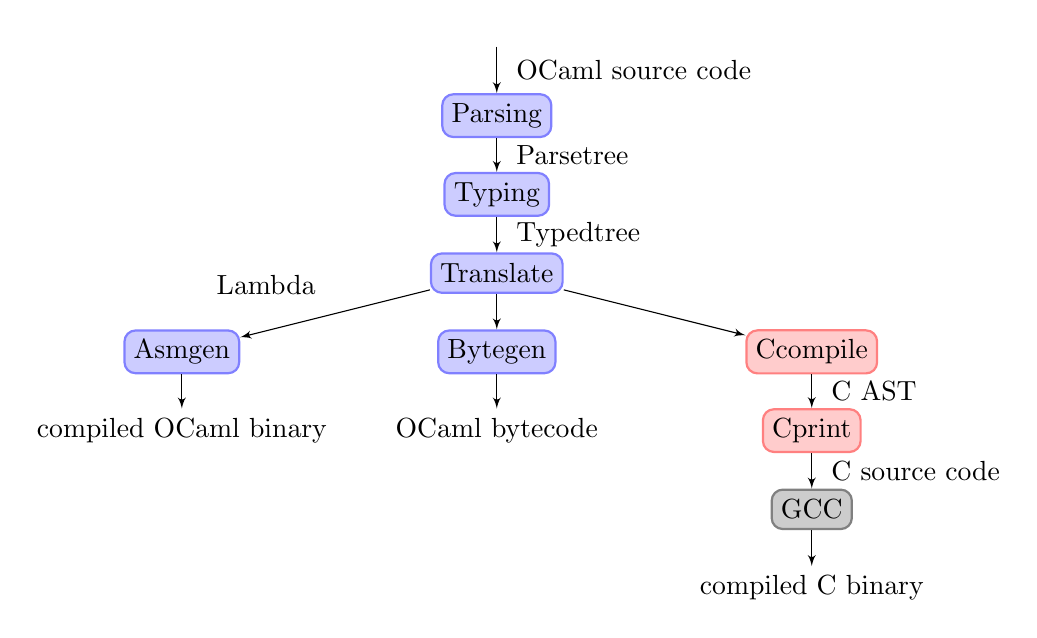
\begin{tikzpicture}

\node [blank] (start) {};
\node [block, below of=start] (parsing) {Parsing};
\node [block, below of=parsing] (typing) {Typing};
\node [block, below of=typing] (translate) {Translate};
\node [block, below of=translate] (bytegen) {Bytegen};
\node [blank, below of=bytegen] (compiled-byte) {OCaml bytecode};
\node [block, left of=bytegen, node distance=4cm] (asmgen) {Asmgen};
\node [blank, below of=asmgen] (compiled-asm) {compiled OCaml binary};
\uncover<2-> {\node [block-emph, right of=bytegen, node distance=4cm] 
(ccompile) {Ccompile};}
\uncover<3-> {\node [block-emph, below of=ccompile] (cprint) {Cprint};}
\uncover <4-> {\node [block-neutral, below of=cprint] (gcc) {GCC};}
\uncover <4-> {\node [blank, below of=gcc] (compiled-gcc) {compiled C 
binary};}

\path [line] (start) -- node [midway, label=right:{OCaml source code}] {}
(parsing);
\path [line] (parsing) -- node [label=right:{Parsetree}] {} (typing);
\path [line] (typing) -- node [label=right:{Typedtree}] {} (translate);
\path [line] (translate) -- node [label=above left:{Lambda}] {} (asmgen);
\path [line] (asmgen) -- (compiled-asm);
\path [line] (translate) -- (bytegen);
\path [line] (bytegen) -- (compiled-byte);
\uncover<2-> {\path [line] (translate) -- (ccompile); }
\uncover<2-> {\path [line] (ccompile) -- node [label=right:{C AST}] {} 
(cprint);}
\uncover <3-> {\path [line] (cprint) -- node [label=right:{C source code}] {} 
(gcc);}
\uncover<4-> {\path [line] (gcc) -- (compiled-gcc);}

\end{tikzpicture}
}
\end{figure}
\end{frame}

\begin{frame}{Completed work so far}
Core project (a subset of OCaml containing the most commonly used features) is 
complete, including:
\begin{itemize}
\pause
\item obtaining types from the Lambda IR
\item writing a representation of a subset of C in OCaml
\pause
\item translation of commonly used language constructs. such as \texttt{let}, 
\texttt{let rec}, \texttt{if}, \texttt{for}, \texttt{while}, \texttt{ref}, 
pattern matching etc.
\item design of algebraic data structure representation and implementation
\item design of closure representation, closure conversion, and function and 
data structure polymorphism
\pause
\item library of toy OCaml programs for testing and benchmarking
\item some evaluation into performance and observability of compiled output
\end{itemize}
\end{frame}

\begin{frame}{Benchmarks}
\begin{figure}
\only<1,3->{
\resizebox{!}{0.9\textheight}{
\includegraphics{benchmark_graph.pdf}
}
}
\only<2>{

\includegraphics[height=0.9\textheight]{mandelbrot.png}
}
\end{figure}
\end{frame}

\begin{frame}[fragile]{Observability Demo}
\begin{lstlisting}[basicstyle=\ttfamily\footnotesize]
(gdb)@\pause@ l@\pause@
1       let sum xs =
2         let rec go acc = function
3           | x :: xs -> go (acc + x) xs
4           | [] -> acc
5         in go 0 xs
6
7       let a = sum [3]
(gdb)@\pause@ tb 2@\pause@
Temporary breakpoint 1 at 0x400690: tests/observability/sum.ml:2. (2 locations)
(gdb)@\pause@ r@\pause@
Starting program: tests/observability/sum 

Temporary breakpoint 1, func_1233 (xs_1205=...) at tests/observability/sum.ml:2
2         let rec go acc = function
(gdb)@\pause@ s@\pause@
5         in go 0 xs
(gdb)@\pause@
local_func_1215 (acc_1207=0, param_1210=..., closure_obj_1214=0x602050) at tests/observability/sum.ml:2
2         let rec go acc = function
\end{lstlisting}
\end{frame}

\begin{frame}[fragile]{Observability Demo}
\begin{lstlisting}[basicstyle=\ttfamily\footnotesize]
(gdb)@\pause@
3           | x :: xs -> go (acc + x) xs
(gdb)@\pause@ p x_1208 @\pause@
$1 = 3
(gdb)@\pause@ p acc_1207@\pause@
$2 = 0
(gdb)@\pause@ p xs_1209@\pause@
$3 = {i = 1, block = 0x1}
(gdb)@\pause@ s@\pause@
local_func_1215 (acc_1207=3, param_1210=..., closure_obj_1214=0x602050) at tests/observability/sum.ml:2
2         let rec go acc = function
(gdb)@\pause@
4           | [] -> acc
(gdb)@\pause@ finish@\pause@
Run till exit from #0  local_func_1215 (acc_1207=3, param_1210=..., closure_obj_1214=0x602050) at tests/observability/sum.ml:4
0x0000000000400740 in local_func_1215 (acc_1207=0, param_1210=..., closure_obj_1214=0x602050) at tests/observability/sum.ml:3
3           | x :: xs -> go (acc + x) xs
Value returned is $4 = 3
(gdb)
\end{lstlisting}
\end{frame}

\begin{frame}{Further work}

The project is roughly on schedule, within 1--2 weeks of the timetable.
\vspace{1em}

Further work on the project would include:
\begin{itemize}
    \pause
    \item Using \texttt{liballocs} and \texttt{gdb} scripts to improve
    `observability' and user experience while debugging
    \pause
    \item Further evaluation tasks into performance and observability
\end{itemize}

\pause
Extension tasks:
\begin{itemize}
    \pause
    \item improving closure creation performance
    \pause
    \item compilation of modules, functors and exceptions
    \pause
    \item compilation of standard library modules
\end{itemize}

\end{frame}

\begin{frame}[fragile]{Some example C code}
\begin{lstlisting}[breaklines=true, language=C,
keywordstyle=\color{keywords},
commentstyle=\color{comments},
stringstyle=\color{strings},
showstringspaces=false,
identifierstyle=\color{identifiers}]
#line 2 "tests/observability/sum.ml"
intptr_t local_func_1215(intptr_t acc_1207,value_type param_1210,closure_t closure_obj_1214){closure_t go_1206;go_1206=TO_CLOSURE(closure_obj_1214[(TO_INT(*(closure_obj_1214))-1)]);
#line 2 "tests/observability/sum.ml"
intptr_t ifelse_return_1216;if(UNBOX_INT(param_1210)){variable_type field_access_1217;field_access_1217=UNBOX_BLOCK(param_1210)[2];intptr_t let_return_1218;{{value_type xs_1209;xs_1209=TO_VALUE(field_access_1217);variable_type field_access_1219;field_access_1219=UNBOX_BLOCK(param_1210)[1];intptr_t let_return_1220;{{intptr_t x_1208;x_1208=TO_INT(field_access_1219);
#line 3 "tests/observability/sum.ml"

#line 3 "tests/observability/sum.ml"
intptr_t binop_result_1221;binop_result_1221=(acc_1207+x_1208);intptr_t temp_1222;temp_1222=binop_result_1221;value_type temp_1223;temp_1223=xs_1209;intptr_t apply_result_1224;apply_result_1224=((intptr_t(*)(intptr_t,value_type,closure_t))((intptr_t(*)(intptr_t,value_type,closure_t))TO_FUNC(go_1206[(TO_INT(*(go_1206))-0)])))(temp_1222,temp_1223,go_1206);let_return_1220=apply_result_1224;}}let_return_1218=let_return_1220;}}ifelse_return_1216=let_return_1218;}else{
#line 4 "tests/observability/sum.ml"
ifelse_return_1216=acc_1207;}intptr_t return_value_1225;return_value_1225=ifelse_return_1216;return return_value_1225;}

#line 1 "tests/observability/sum.ml"
intptr_t func_1233(value_type xs_1205){
#line 1 "tests/observability/sum.ml"

#line 2 "tests/observability/sum.ml"
closure_t go_1206;go_1206=MALLOC((sizeof(variable_type)*3));intptr_t(*temp_1226)(intptr_t,value_type,closure_t);temp_1226=&(local_func_1215);closure_t closure_obj_1227;closure_obj_1227=MALLOC((sizeof(variable_type)*3));closure_obj_1227[0]=FROM_INT(2);closure_obj_1227[1]=FROM_CLOSURE(go_1206);closure_obj_1227[2]=FROM_FUNC(temp_1226);MEMCPY(go_1206,closure_obj_1227,3);
#line 5 "tests/observability/sum.ml"

#line 5 "tests/observability/sum.ml"
intptr_t const_1228;const_1228=0;intptr_t temp_1229;temp_1229=const_1228;value_type temp_1230;temp_1230=xs_1205;intptr_t apply_result_1231;apply_result_1231=((intptr_t(*)(intptr_t,value_type,closure_t))((intptr_t(*)(intptr_t,value_type,closure_t))TO_FUNC(go_1206[(TO_INT(*(go_1206))-0)])))(temp_1229,temp_1230,go_1206);intptr_t return_value_1232;return_value_1232=apply_result_1231;return return_value_1232;}
\end{lstlisting}
\end{frame}

\end{document}
